\documentclass{sig-alternate}
\usepackage{tabularx}
\usepackage[noabbrev]{cleveref}
\usepackage{times}

\begin{document}

% Copyright
\setcopyright{acmcopyright}
%\setcopyright{acmlicensed}
%\setcopyright{rightsretained}
%\setcopyright{usgov}
%\setcopyright{usgovmixed}
%\setcopyright{cagov}
%\setcopyright{cagovmixed}


% DOI
%\doi{10.475/123_4}

% ISBN
%\isbn{123-4567-24-567/08/06}

%Conference
%\conferenceinfo{PLDI '13}{June 16--19, 2013, Seattle, WA, USA}

%\acmPrice{\$15.00}

%
% --- Author Metadata here ---
\conferenceinfo{MSR}{'16 Austin, Texas USA}
% --- End of Author Metadata ---

\title{The evolution of the GHTorrent: growing an open access dataset}
\numberofauthors{1} %  in this sample file, there are a *total*
% of EIGHT authors. SIX appear on the 'first-page' (for formatting
% reasons) and the remaining two appear in the \additionalauthors section.
%
\author{
% The command \alignauthor (no curly braces needed) should
% precede each author name, affiliation/snail-mail address and
% e-mail address. Additionally, tag each line of
% affiliation/address with \affaddr, and tag the
% e-mail address with \email.
%
% 1st. author
\alignauthor Georgios Gousios\\
       \affaddr{Radboud University Nijmegen}\\
       \affaddr{Nijmegen, the Netherlands}\\
       \email{g.gousios@cs.ru.nl}
}

\maketitle
\begin{abstract}

With over 31 million repositories and 12 million users, GitHub is by far the
biggest open source forge in existense. Since early 2012, the GHTorrent project
has been retrieving data from GitHub's open access API and offering them to the
repository mining community.  In this paper, we describe how we grew GHTorrent
to 10x the size of early 2013, while at the same time improving its coverage,
quality and versatility and offering data access services to hundrends of
researchers.

\end{abstract}

%
% The code below should be generated by the tool at
% http://dl.acm.org/ccs.cfm
% Please copy and paste the code instead of the example below. 
%
\begin{CCSXML}
<ccs2012>
 <concept>
  <concept_id>10010520.10010553.10010562</concept_id>
  <concept_desc>Computer systems organization~Embedded systems</concept_desc>
  <concept_significance>500</concept_significance>
 </concept>
 <concept>
  <concept_id>10010520.10010575.10010755</concept_id>
  <concept_desc>Computer systems organization~Redundancy</concept_desc>
  <concept_significance>300</concept_significance>
 </concept>
 <concept>
  <concept_id>10010520.10010553.10010554</concept_id>
  <concept_desc>Computer systems organization~Robotics</concept_desc>
  <concept_significance>100</concept_significance>
 </concept>
 <concept>
  <concept_id>10003033.10003083.10003095</concept_id>
  <concept_desc>Networks~Network reliability</concept_desc>
  <concept_significance>100</concept_significance>
 </concept>
</ccs2012>
\end{CCSXML}

\ccsdesc[500]{Computer systems organization~Embedded systems}
\ccsdesc[300]{Computer systems organization~Redundancy}
\ccsdesc{Computer systems organization~Robotics}
\ccsdesc[100]{Networks~Network reliability}


%
%  Use this command to print the description
%
\printccsdesc

\keywords{ACM proceedings; \LaTeX; text tagging}

\section{Introduction}


\section{Current status}

\begin{table}
  \centering
  \begin{small}
  \label{tab:datasetsize}
  \begin{tabular}{llll}
    \hline
    \bfseries{Entity} & \bfseries{MongoDB} & \bfseries{MySQL} & \bfseries{Diff to 2013} \\
    \hline
      Events                     & 476,047,453 & ---           & 11.1x\\
      Users                      & 6,733,244   & 9,277,113     & 8.4x \\
      \ldots of which fake       & ---         & 2,435,859     & ---\\
      \ldots of which deleted    & ---         & 271,590       & ---\\
      \ldots of which geolocated & ---         & 1,108,784     & \\
      Repositories               & 28,851,321  & 25,578,419    & 21.8x\\
      \ldots of which forks      & ---         & 10,486,114    & --- \\
      \ldots of which deleted    & ---         & 4,986,095     & ---\\
      Commits                    & 367,815,284 & 362,057,838   & 12.3x \\
      Issues                     & 24,165,582  & 25,351,996    & 10.3x \\
      Pull requests              & 11,944,969  & 11,114,625    & 9.7x \\
      Issue comments             & 42,021,374  & 43,416,372    & 14.6x\\
      Watchers (stars)           & 51,698,373  & 37,022,681    & 6.6x\\
      \hline
  \end{tabular}
    \caption{GHTorrent database contents as of Jan 14, 2016. The difference column reports the difference to the numbers reported in reference ~\cite{Gousi13}.}
  \end{small}
\end{table}

\subsection{Repositories}

\subsubsection{Better project descriptions}


\subsubsection{All project languages are retrieved}
GitHub maintains a 


\subsubsection{Forks}

When a project is forked, GitHub will create an identical copy of the project
repository and initialize a new issue tracker for it. Internally, the repository
contents are not really duplicated; GitHub will use a copy-on-write
mechanism to minimize disk space use.\footnote{http://githubengineering.com/counting-objects/} This process makes forking very cheap for GitHub.

When GHTorrent encounters a fork event, it treats the fork as a new repository.
It thus recursively retrieves all information about the fork, such as the
repository owner and issue labels. In the early versions of
GHTorrent, recursive retrieval also included commits. For big and popular
projects, such as Ruby on Rails (55k commits, 11k forks),
this process required several (thousand) additional GitHub API calls, which
quickly depleted GHTorrent limited API rates. For this reason, GHTorrent implemented a mechanism that only retrieve new commits from forks until
it found a shared commit with the parent repository; it would then switch
to copying commits internally within the GHTorrent database. This trick worked
with formidable efficiency, as it cut down on API calls (and the time required
to process them) by more than 95\% for big projects.

However, its very efficiency caused a new problem; \emph{too many} forks where
processed meant that the table that records the association between commits and
repositories (\texttt{project\_\-commits}) grew uncontrollably. Just for Ruby on
Rails, this table would store more than 500M rows. The root of the problem
is that \texttt{project\_commits} models an $M \times N$ relationship between
projects and commits and this cannot be normalized further without signicant
duplication (Boyce-Codd Normal form).

Concequently, retrieving fork commits was converted to an optional
configuration parameter and are not retrieved by default. Therefore, the
(\texttt{project\_\-commits}) table is inconsistent with respect to
fork commits.

\subsection{Users}
\subsubsection{Better user identification}

When a commit is being processed by GHTorrent, a user must be associated with it.
GHTorrent first attempts to query GitHub for information about the committer
and, if this fails (the committer is not registered with GitHub), then it
creates a fake user to register this commit with. Until recently, it was not
possible to identify fake users; GHTorrent now marks them as such in the MySQL
database. Moreover, it can convert fake users to normal users if a user with
the provided email is registered with GitHub in the future.

Moreover, similarily to projects, users can also delete their accounts.
GHTorrent keeps track of deleted users by marking them as such. This helps
researchers to eliminate inactive users from their analyses.

\subsubsection{Geolocation}

Almost 1.3M GitHub users share their location in their profiles. GHTorrent uses
this information to \emph{geolocate} those users. Geolocation refers to the
process of converting a text string potentially indicating the address of a
place on earth to the longitude and latitude co-ordinates corresponding to this
address. As GitHub's address field is free-form text, there are no guarantees
about the format of the address fields. GHTorrent uses the OpenStreetMap
geolocation service (Nominatim) for this functionality. To overcome Nomitatim's
API restrictions, it caches geolocated places in the Mongo database. 160,000
cached addresses have been collected so far, with a very high cache hit ratio.
An example application of geolocation information can be seen in
Figure~\ref{fig:dev-map}.

It is important to notice that geolocation in GHTorrent is a best effort
approach. Initially, not all user provided location strings can be decoded to a
real address; on the one hand, several users provide fictional addresses while
on the other the Nominatim service is not top of the crop for geolocation.
Moreover, users may choose not to share their addresses while cultural
differences in online privacy perceptions may lead to whole clusters of users
being under-respresented. Concequently, care must be applied when drawing
conclusions from this data.

\begin{figure}
  \begin{center}
    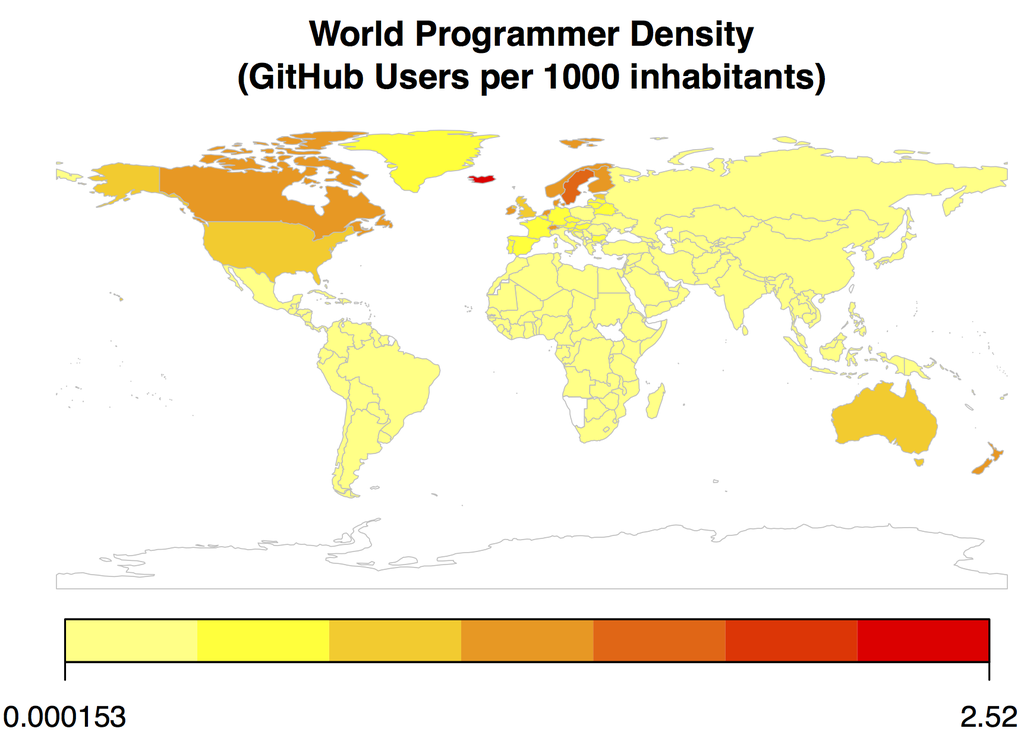
\includegraphics[scale=0.2]{dev-map.png}
  \end{center}
  \caption{GHTorrent users that registered a location plotted on a map after
  geocoding them.}
  \label{fig:dev-map}
\end{figure}

\subsection{Service}

\subsubsection{Lean GHTorrent is discontinued}


\subsubsection{Shared data}
Weekly MySQL dumps, daily mongoDb dumps
\subsection{Online access to databases}
Mongo, MySQL, Juniper setup with MySQL/Mongo
\subsection{Service monitoring}

\section{Open research topics}

\section{Conclusions}

\section*{Acknoweledgements}

The GHTorrent project would like to thank Microsoft for their generous support
that enabled the move to the Azure cloud. The author would also like the
numerous GHTorrent users (Bogdan Vasilescu and Daniel German require special
mention) for the fruitful discussions that led to a better GHTorrent for
everybody.

\bibliographystyle{acm}
\bibliography{ghtorrent-update}


\end{document}
